%This is a test file to determine the layout of the Owl Datasheet
\documentclass{article}
\pagestyle{myheadings}
\markright{BBa\_J23100}
\usepackage[xcolor]{mdframed} %Top header has banner!
\usepackage{hyphenat} %Column titles are not to have hyphenation
\usepackage{seqsplit} %Manages long DNA sequence line breaks
\usepackage{ccaption} %Formatting table titles
\usepackage[margin=1in]{geometry} %Setting document margins
\usepackage{graphicx} %Using images
\usepackage{array} %Formatting table size and behavior
\begin{document}
\renewcommand{\topfraction}{0.99} %Helps with keeping whitespace to a minimum
\renewcommand{\textfraction}{0.99}
\renewcommand{\floatpagefraction}{0.99}
\begin{table}[htbp]
\setlength{\belowcaptionskip}{4pt}
\setlength{\extrarowheight}{8pt}
\begin{mdframed}[backgroundcolor=gray!32,topline=false,rightline=false,leftline=false,bottomline=false] \legend{\Huge \underline{BBa\_J23100}} \end{mdframed} \hfill \break
\begin{tabular}{m{1.2in}m{4.98in}}
\large \textbf{\nohyphens{Part Summary}} & Parts J23100 through J23119 are a family of constitutive promoter parts isolated from a small combinatorial library. J23119 is the consensus promoter sequence and the strongest member of the family. All parts except J23119 are present in plasmid J61002. Part J23119 is present in pSB1A2. This places the RFP downstream of the promoter. Reported activities of the promoters are given as the relative fluorescence of these plasmids in strain TG1 grown in LB media to saturation. See part J61002 for details on their use. These promoter parts can be used to tune the expression level of constitutively expressed parts. The NheI and AvrII restriction sites present within these promoter parts make them a scaffold for further modification.\\
\large \textbf{\nohyphens{Sequence}} & \seqsplit{ttgacggctagctcagtcctaggtacagtgctagc}\\
\large \textbf{\nohyphens{Part Type}} & Basic Part\\
\large \textbf{\nohyphens{Related Parts}} & J23101, J23102, J23103, J23104, J23105, J23106, J23107, J23108, J23109, J23110, J23111, J23112, J23113, J23114, J23115, J23116, J23117, J23118, J23119\\
\large \textbf{\nohyphens{Pigeon Image}} & \hfill \break 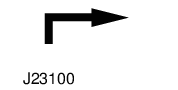
\includegraphics[width=10cm,height=10cm,keepaspectratio]{/Users/Zach/Documents/Owl/igem-datasheet/Datasheet_Generator/src/main/webapp/tmp/1439916848319BBa_J23100_pigeon.png} \\ 
\large \textbf{\nohyphens{Plasmid Map}} & \hfill \break 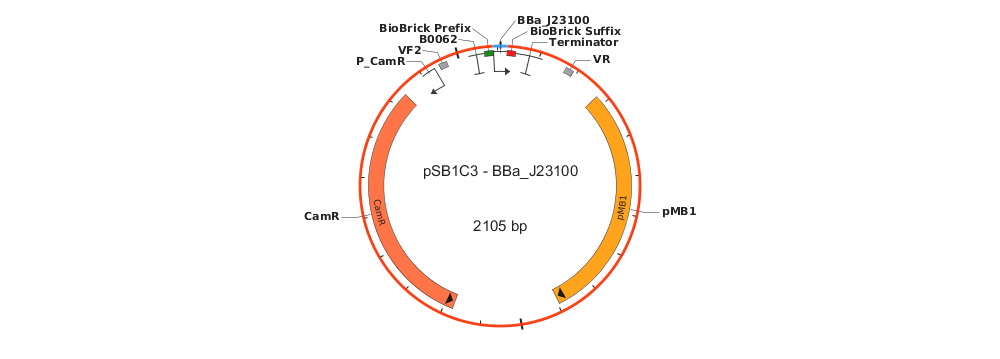
\includegraphics[width=10cm,height=10cm,keepaspectratio]{/Users/Zach/Documents/Owl/igem-datasheet/Datasheet_Generator/src/main/webapp/tmp/1439916848431BBa_J23100_plasmid_map.png} \
\end{tabular}
\end{table}
\begin{table}[htbp]
\setlength{\belowcaptionskip}{4pt}
\setlength{\extrarowheight}{8pt}
\begin{mdframed}[backgroundcolor=gray!32,topline=false,rightline=false,leftline=false,bottomline=false] \legend{\LARGE Designer Information}\end{mdframed}
\begin{tabular}{m{1.2in}m{4.98in}}
\large \textbf{\nohyphens{Author(s)}} & J. Christopher Anderson\\
\large \textbf{\nohyphens{Date}} & \seqsplit{2006-08-04}\\
\large \textbf{\nohyphens{Affiliation}} & University of California, Berkeley\\
\large \textbf{\nohyphens{Team}} & \seqsplit{iGEM2006\_Berkeley}\\
\large \textbf{\nohyphens{Contact}} & \seqsplit{jcanderson@berkeley.edu}
\end{tabular}
\end{table}
\begin{table}[htbp]
\setlength{\belowcaptionskip}{4pt}
\setlength{\extrarowheight}{8pt}
\begin{mdframed}[backgroundcolor=gray!32,topline=false,rightline=false,leftline=false,bottomline=false] \legend{\LARGE Design Details}\end{mdframed}
\begin{tabular}{m{1.2in}m{4.98in}}
\large \textbf{\nohyphens{Type}} & Constitutive promoter\\
\large \textbf{\nohyphens{Vector}} & \seqsplit{pSB1C3}
\end{tabular}
\end{table}
\begin{table}[htbp]
\setlength{\belowcaptionskip}{4pt}
\setlength{\extrarowheight}{8pt}
\begin{mdframed}[backgroundcolor=gray!32,topline=false,rightline=false,leftline=false,bottomline=false] \legend{\LARGE Assembly Information}\end{mdframed}
\begin{tabular}{m{1.2in}m{4.98in}}
\large \textbf{\nohyphens{Assembly Method(s)}} & \seqsplit{BioBricks}\\
\large \textbf{\nohyphens{Chassis}} & Escherichia coli\\
\large \textbf{\nohyphens{Assembly RFC}} & \seqsplit{10}\\
\large \textbf{\nohyphens{Scars}} & \seqsplit{yes}
\end{tabular}
\end{table}
\end{document}
